\section{Einführung}
\label{sec:intor}

Die vorliegende Aufgabe dreht sich um die Systemidentifikation zweier System.
Dafür wurden in der Aufgabenstellung jeweils ein FIR und ein IIR Filter gegeben.
Mit Hilfe der in der Vorlesung besprochenen adaptiven Filter sollte die Koeffizienten der gegebenen System identifiziert werden.
Als Vorbereitung auf die Systemidentifikation wurden der Least-Mean-Square Algorithmus (LMS) und der Recursive-Least-Squares Algorithmus mit Vergessenfaktor (RLS) implementiert.
Die Implementation erfolgte in Python \footnote{Software Repository:\url{https://github.com/Foaly/AdaptiveFilter}} anhand der Rechenvorschrift nach [Moschytz] \footnote{George Moschytz and Markus Hofbauer. Adaptive Filter: Eine Einführung in die Theorie mit Aufgaben und MATLAB-Simulationen auf CD-ROM (German Edition). Springer, 2000 edition, 10 2000.} (LMS nach S. 85 und RLS nach S.145).

\section{FIR-Filter}
\label{sec:fir}

Die erste Aufgabe ist die Systemidentifikation eines FIR Filters mit 5 Koeffizienten.
Das System wird mit Hilfe des LMS und KLS (mit Vergessensfaktor) Algorithmus identifiziert.
Der Einfluss unterschiedlicher Parameter, wie die Anzahl der Filterkoeffizienten, die Varianz des hinzugefügten Rauschens und die Werte für Schrittweite oder Vergessensfaktor auf das Ergebnis wird dabei untersucht.

\subsection{Anzahl an Filterkoeffizienten}

Die Anzahl der Filterkoeffizienten ist einer der Parameter, der die Systemidentifikation am Stärksten beeinflusst. 
Zu erwarten wäre, dass sich das zu identifizierende System mit weniger Koeffizienten als nötig nicht hinreichend genau abbilden lässt. 
Dies erweist sich auch als korrekt.
Dabei fällt auf, dass dem LMS Algorithmus die Approximation mit zu wenig Filterkoeffizienten wesentlich besser gelingt, als der RLS Algorithmus (vgl. die beiden Plots in \ref{fig:N1} und \ref{fig:N2}).

\begin{figure}[H]
  \centering
      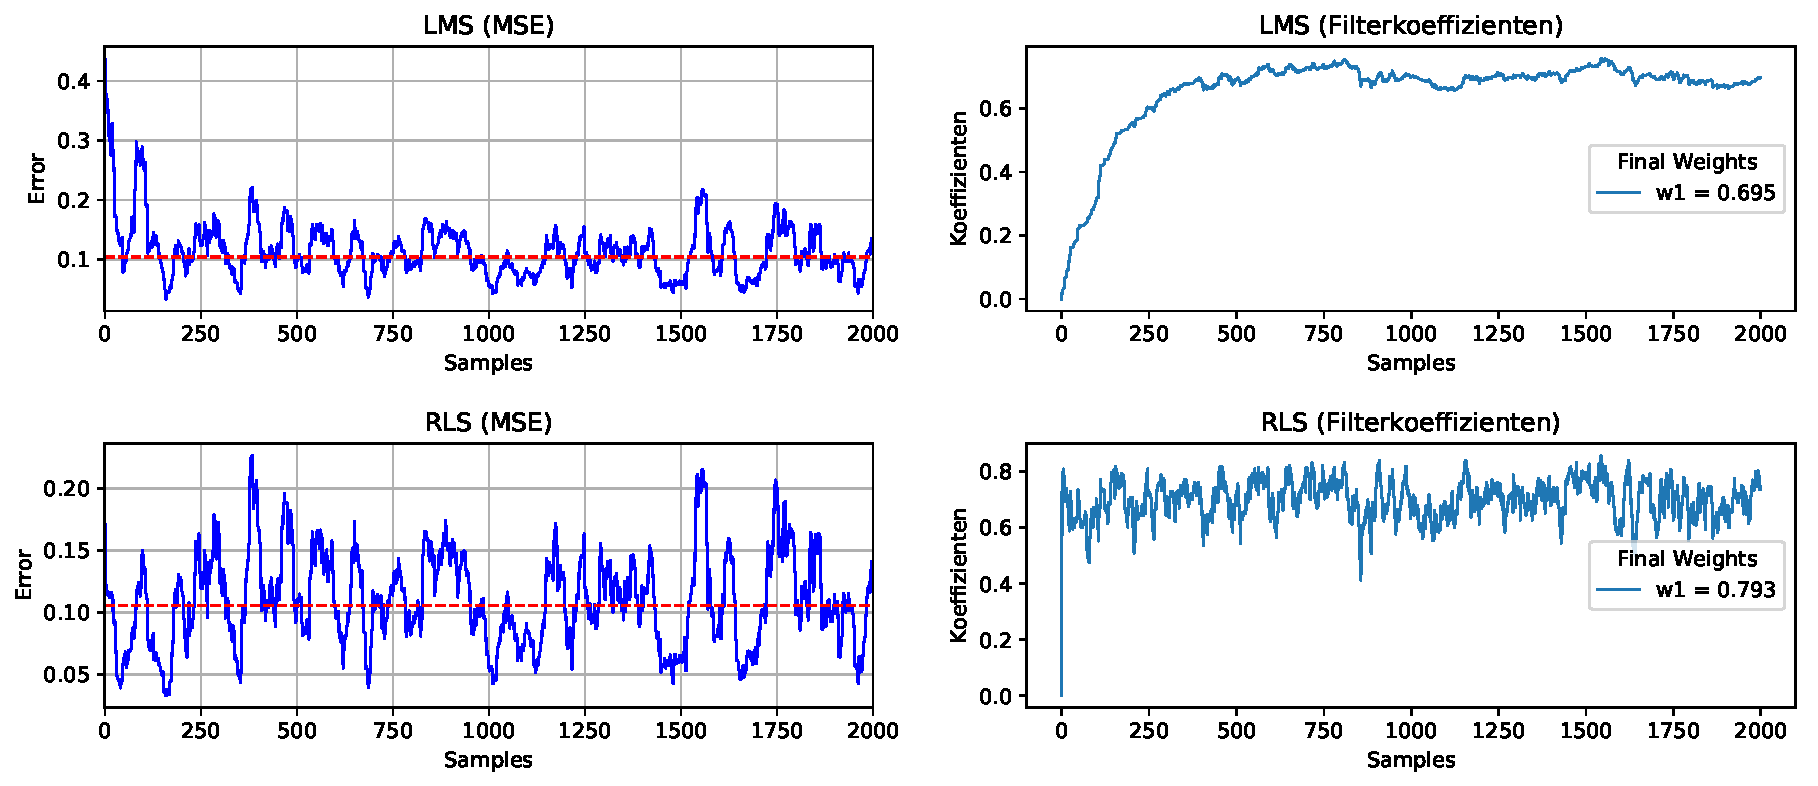
\includegraphics[width=0.6\textwidth]{{{figures/N_1_var_0.001}}}
 \caption{Vergleich zwischen LMS und RLS mit je einem Filterkoeffizienten (N=1)}
	\label{fig:N1}
\end{figure}

\begin{figure}[H]
  \centering
      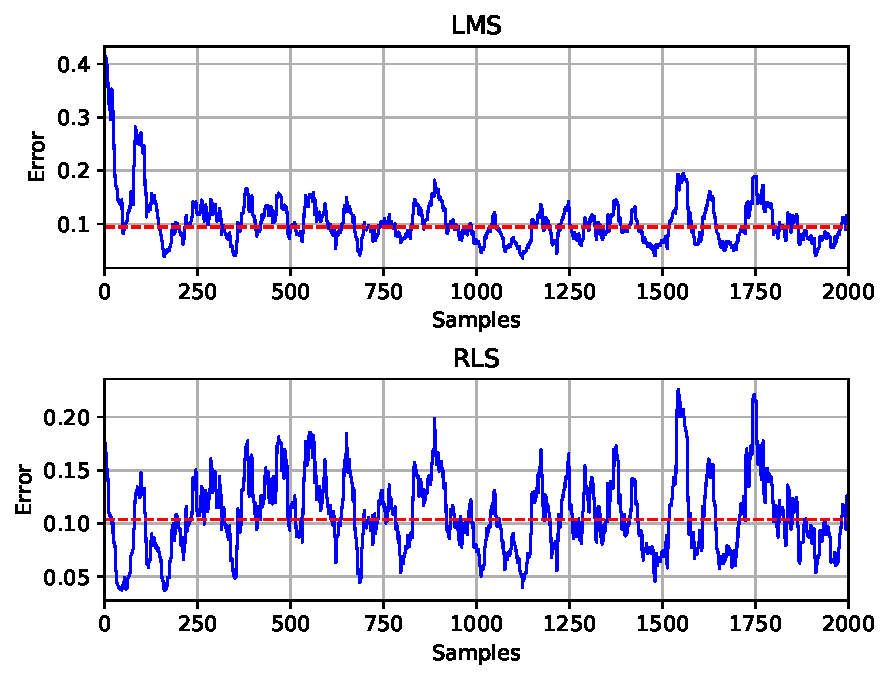
\includegraphics[width=0.6\textwidth]{{{figures/N_2_var_0.001}}}
 \caption{Vergleich zwischen LMS und RLS mit je zwei Filterkoeffizienten (N=2)}
	\label{fig:N2}
\end{figure}

\begin{figure}[H]
  \centering
      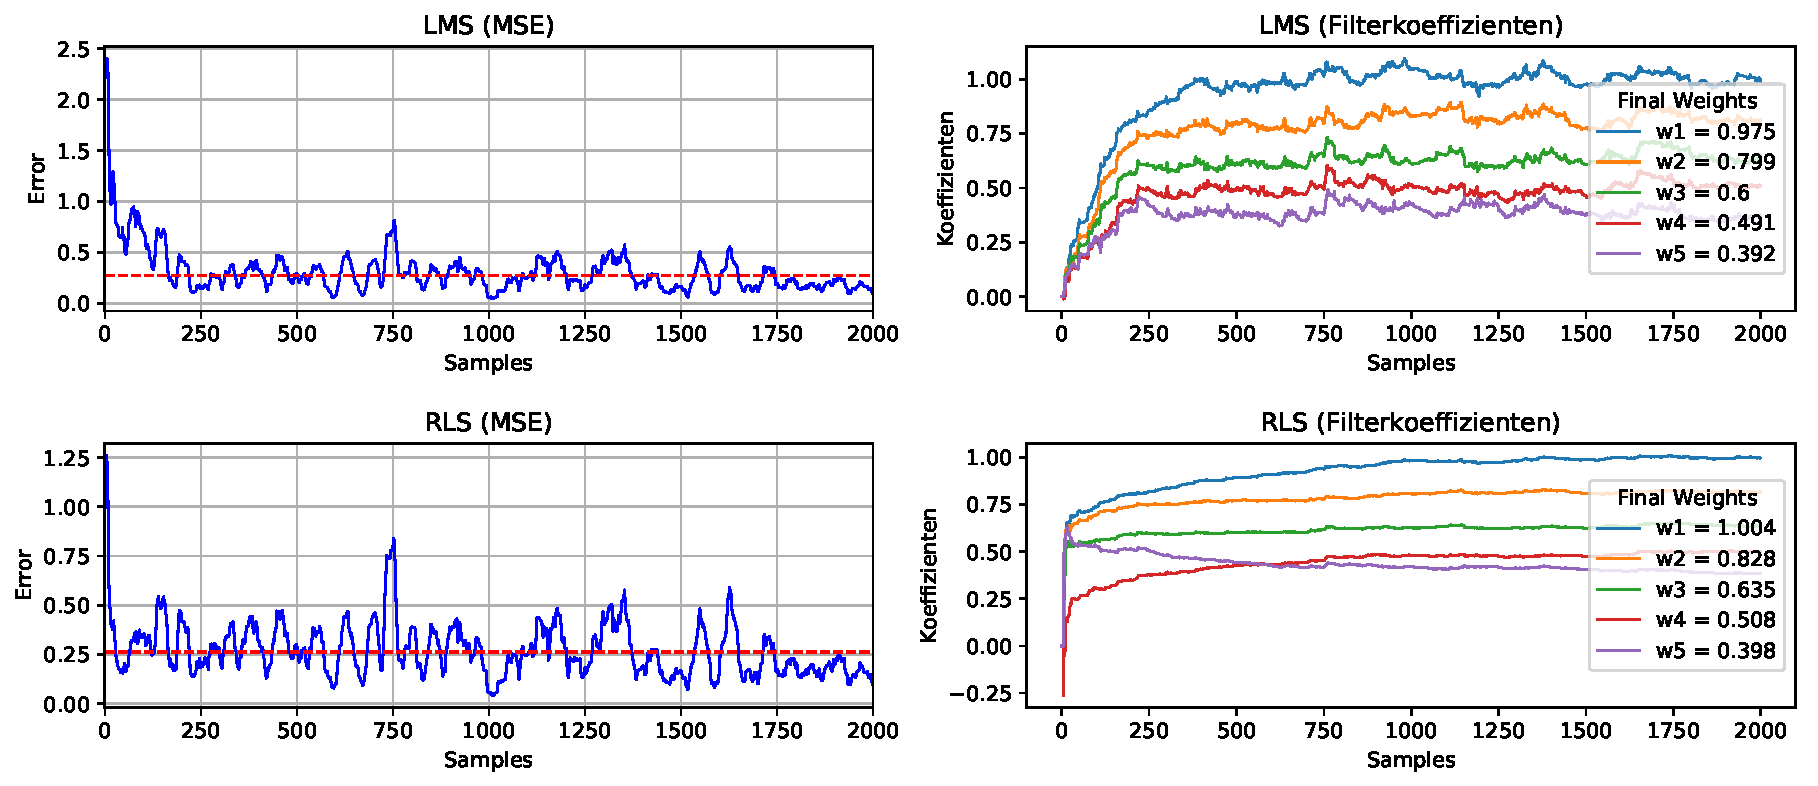
\includegraphics[width=0.6\textwidth]{{{figures/N_5_var_0.001}}}
 \caption{Vergleich zwischen LMS und RLS mit je fünf Filterkoeffizienten (N=5)}
	\label{fig:N5}
\end{figure}



\subsection{Wahl des Lernalgorithmus}
\subsection{Einfluss der Varianz}
\files{main.py}


\section{IIR-Filter}
\label{sec:iir}

\subsection{Anzahl an Filterkoeffizienten}
\subsection{Wahl des Lernalgorithmus}
\subsection{Einfluss der Varianz}


\section{Systemwechsel}
\label{sec:3}

\subsection{Adaptionsverhalten}


\section{Kernel Least Mean Squares}
\label{sec:3}


\section{Fehlerfunktion(en)}